\documentclass{article}
\pagestyle{empty}
%\usepackage{geometry,fontspec,tikz}
\usepackage[svgnames]{xcolor}
\usepackage{geometry,tikz}
\newcommand{\h}[1]{\textcolor{FireBrick}{#1}}
\geometry{a6paper,landscape,hmargin={1cm,1cm},vmargin={1cm,1cm}}
%\setmainfont[Ligatures=TeX]{Adobe Garamond Pro}
\usetikzlibrary{fadings}
\tikzfading[name=fade right,
left color=transparent!0,
right color=transparent!100]
\setlength\parindent{0pt}
\begin{document}
\begin{tikzpicture}[overlay,remember picture]
  \node[anchor=east,inner sep=0pt] (pic) at (current page.east)
    {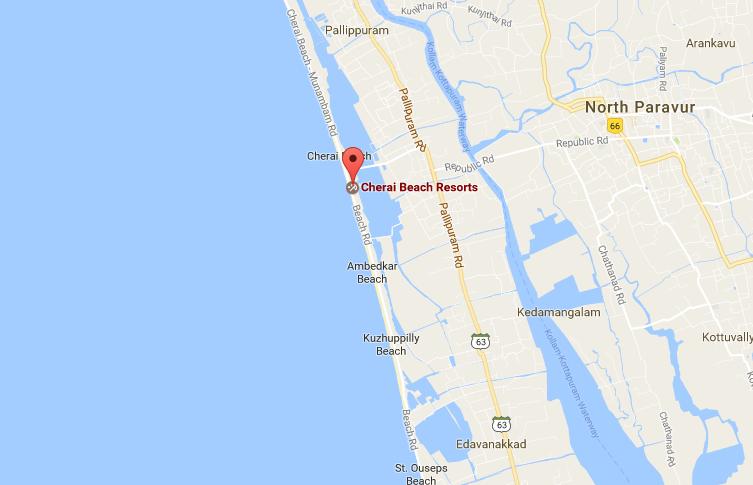
\includegraphics[width=\paperwidth,height=\pdfpageheight]{map}};
  \fill[white,path fading=fade right] (pic.north west) rectangle (pic.south east);
  \coordinate (pin) at (5.95,-2.4);
  \filldraw[ultra thick,draw=red,fill=red!20] (pin) -- ++(70:.5) arc (-20:200:.18) -- cycle;
  \path (pin) -- ++(0,.5) node[draw,fill,red,circle,inner sep=1pt] {};
\end{tikzpicture}%
\obeylines%
%{\addfontfeatures{Scale=3,LetterSpace=10} INVITATION}
{\huge{\textsc{\h{V}enue}}}
\bigbreak
{\small \emph\textit{%
\textsc{\h{C}herai \h{B}each \h{R}esorts}
Vypin Island
Kochi, Kerala
Pin - 683514 
}}

\vfill

%{\addfontfeatures{Scale=1.4,LetterSpace=5}\scshape when?}
{\scshape \h{W}hen?}
{\small \emph \textit{%
  \scshape June 10\/\rlap{,}\textsuperscript{th} 2017
  11\kern.5pt:\kern.5pt30 am
}}
\medbreak
%{\addfontfeatures{Scale=1.4,LetterSpace=5}\scshape where?}
{\scshape \h{D}irections?}
\textit{%
  Times Square,
  London E1,
  UK
}
\end{document}